\documentclass[./main.tex]{subfiles}


\begin{document}
    \subsubsection*{問1}
    \addcontentsline{toc}{subsubsection}{問1}
    \markboth{2023年 統計数理 問1}{2023年 統計数理 問1}

    \begin{enumerate}
        % Q1
        \item $E[X] = \displaystyle\sum_{x=0}^\infty x \cdot \frac{\lambda^x}{x!} e^{- \lambda}
            = \lambda e^{-\lambda} \sum_{x=1}^\infty \frac{\lambda^{x-1}}{(x - 1)!} = \lambda.$\\
        $E[X (X - 1)] = \displaystyle \sum_{x=0}^\infty x (x - 1) \cdot \frac{\lambda^x}{x!} e^{-\lambda}
            = \lambda^2 e^{-\lambda} \sum_{x=2}^\infty \frac{\lambda^{x - 2}}{(x - 2)!} = \lambda^2.$\\
        $\therefore \ V[X] = E[X (X - 1)] + E[X] - E[X]^2 = \lambda.$\\
        $X_1, \dots, X_n$ は iid なので、$E[S_n] = n \lambda$, $V[S_n] = n\lambda.$

        % Q2
        \item $\displaystyle W_n = \sum_{k=1}^n \sum_{i=1}^k X_i$ を展開した時に現れる $X_i$ の個数を数えることで、$a_i = n + 1 - i \ (i = 1, \dots, n)$.

        % Q3
        \item $E [W_n] = \displaystyle \sum_{i=1}^{n} (n + 1 - i) E [X_i] = \frac{\lambda}{2} n(n + 1)$,\\
        $V[W_n] = \displaystyle \sum_{i=1}^n (n + 1 - i)^2 V[X_i] = \frac{\lambda}{6} n (n + 1) (2n + 1).$

        % Q4
        \item 例えば $\displaystyle \tilde{\lambda} = \dfrac{2}{n(n+1)} W_n$ とすると [3] の結果から $E[\tilde{\lambda}] = \lambda$ と不偏になる。
        このとき\\
            $\displaystyle V[\tilde{\lambda}]
                = \left\{ \frac{2}{n (n + 1)} \right\}^2 V [W_n]
                = \left\{ \frac{2}{n (n + 1)} \right\}^2 \cdot \frac{\lambda}{6} n (n + 1) (2n + 1)
                = \frac{2 \lambda}{3} \frac{(2n + 1)}{n (n + 1)} .$
        
        % Q5
        \item $\forall \varepsilon > 0$ を任意にとると、チェビシェフの不等式より
        \begin{equation*}
            P (\vert \tilde{\lambda} - \lambda \vert \geq \varepsilon)
                \leq \frac{V[\tilde{\lambda}]}{\varepsilon^2}
                = \frac{2\lambda}{3 \varepsilon^2} \frac{(2n + 1)}{n (n + 1)} 
                \to 0 \quad (n \to \infty)
        \end{equation*}
        したがって、$\tilde{\lambda}$ は $\lambda$ の一致推定量である。

        % Q6
        \item $V[\hat{\lambda}] = \dfrac{1}{n^2} V[S_n] = \dfrac{\lambda}{n}$ より、$\tilde{\lambda}$ の $\hat{\lambda}$ に対する漸近相対効率は
        \begin{equation*}
            \lim_{n \to \infty} \frac{V [ \hat{\lambda}]}{V [ \tilde{\lambda} ]}
                = \lim_{n \to \infty}
                    \frac{\lambda}{n} \cdot \frac{3}{2\lambda}\frac{n (n + 1)}{(2n + 1)} 
                = \frac{3}{4}.
        \end{equation*}


    \end{enumerate}
    \subsubsection*{コメント}
    あなた、漸近相対効率を知っていますか?という問題です。
    定義載せてくれ定期
    \begin{enumerate}
        \item 色々やり方はあると思います。
        分散を求める時に、定義 $E[(X - \lambda)^2]$ や $E[X^2]$ ではなく $E[X(X - 1)]$ を計算するのは割と常套テクニックですね。
        二項分布や幾何分布等、活躍の機会は多いです。
        \item どこまで記述するか悩みますね。二重和はいざ言語化して説明しようとすると結構難しいです。
        $S_1$ が $n$ 個, $S_2$ が $n - 1$ 個、...、$S_n$ が $1$ 個となっていることが伝われば十分だと思います。
        \item $\displaystyle \sum$ の中身をそのまま展開して公式に当てはめると沼ります。
        [2] で見たように、ここでは $n$ から $1$ についての和になっているので、和の順番が逆になっているだけです。
        \item とりあえず [3] を使えば不偏なものは見つかります。分散の値も流用できます。
        \item 一致性といえば確率収束、確率収束といえばチェビシェフ不等式。
        2022 年の統計応用 (理工学) 問 1 にもチェビシェフ不等式を使う問題が出てましたね。

        チェビシェフ不等式はマルコフの不等式の特殊な場合として示されることが多いですが、
        絵を描いて直接確認することもできます。
        $\forall \varepsilon > 0$ を任意の正の数とし、 $X$ を実数値確率変数とします。
        図 \ref{fig:2023-suri-1-chebyshev} のように $X - E[X]$ を横軸に取った座標平面上に
        2 次関数 $\dfrac{1}{\varepsilon^2} ( X - E[X])^2 $ と
        指示関数 $1_{\{ \vert X - E[X] \vert \geq \varepsilon \}}$ を重ねてみると
        \begin{equation*}
            1_{ \{ \vert X - E[X] \vert \geq \varepsilon \}}
                \leq \frac{1}{\varepsilon^2} (X - E[X])^2
        \end{equation*}
        が常に成り立っていることが分かります。
        これの両辺の期待値をとることで直ちにチェビシェフ不等式
        \begin{equation*}
            P( \vert X - E[X] \vert \geq \varepsilon)
                \leq \frac{V [X]}{\varepsilon^2}
                \qquad (\forall \varepsilon > 0)
        \end{equation*}
        が得られます。
        この議論は必ずしも正確とは言えないかもしれませんが、忘れた時に思い出すタネくらいにはなるような気はします。

        % TikZ さんはいりま~す
        \begin{figure}[tb]

            \centering
            \begin{tikzpicture}[scale=2]
                % 原点
                \draw (0, 0) node [below left] {O};
                % 軸
                \draw[-stealth, thick] (-2, 0) -- (2, 0) node [right] {$X - E[X]$};
                \draw[-stealth, thick] (0, -0.5) -- (0, 2.5);

                % 座標
                \draw (1, 0) node [below] {$\varepsilon$};
                \draw (-1, 0) node [below] {$-\varepsilon$};

                % plot
                \draw[ultra thick, domain={-sqrt(2.5)}:{sqrt(2.5)}, red] plot (\x, {pow(\x, 2)}) node [below right] {$\dfrac{1}{\varepsilon^2} \left( X - E[X] \right)^2$};

                \draw[ultra thick, blue] (-2, 1) -- (-1, 1) -- (-1, 0) -- (1, 0) -- (1, 1) --  (2, 1) node [above] {$1_{ \{ \vert X - E[X] \vert \geq \varepsilon \}}$};

            \end{tikzpicture}
            \caption{チェビシェフ不等式の証明に用いる図}
            \label{fig:2023-suri-1-chebyshev}
        \end{figure}

        \item 漸近 $\displaystyle \left( \lim_{n\to\infty} \right)$、 相対効率 $\displaystyle \left( \frac{V[\hat{\lambda}]}{V[\tilde{\lambda}]} \right)$ ですね。 

    \end{enumerate}
\end{document}